\clearpage
\section{Four-hospital evaluation with source-locked operating points}\label{app:external}

We applied the exported Xiehe classifiers to all 698,502 labeled windows from four external hospitals. Seed 3 used epoch 3 and threshold 0.91; seed 42 used epoch 9 and threshold 0.87. We retained the source preprocessing, PID tables and drift references. No target-site data were used to fit or select weights, epochs or thresholds.

The native baseline uses source epochs 2 and 5 (thresholds 0.81 and 0.82). The four-view, history-matched baseline uses epochs 13 and 8 (0.81 and 0.83). The refreshed-pair predecessor uses epochs 5 and 4 (both 0.95). We recomputed both baselines and matched the historical raw-input predictions to the same manifests, row order, labels and locked checkpoints \citep{predecessor}. All decisions use $p>t$.

\begin{table}[ht]
\caption{External positive-class F1 (\%). Each cell averages seed-specific F1. The final rows weight hospitals equally or pool their confusion counts within seed. Gain and its paired 95\% folder interval are in points versus the predecessor.}\label{tab:external-overview}
\centering\small
\begin{tabular}{@{}lrrrrrrr@{}}
\toprule Site & Windows (positive) & Baseline & Matched & Predecessor & T-MoE & Gain & 95\% interval\\ \midrule
\inputrows tables/external_overview.tex
\bottomrule
\end{tabular}
\end{table}

\begin{table}[ht]
\caption{T-MoE at its source-selected thresholds. Precision, recall, F1, average precision (AP) and AUROC are percentages.}\label{tab:external-operating}
\centering\small
\begin{tabular}{@{}lrrrrrrrrrr@{}}
\toprule Site & Seed & TP & FP & FN & TN & Precision & Recall & F1 & AP & AUROC\\ \midrule
\inputrows tables/external_operating.tex
\bottomrule
\end{tabular}
\end{table}

We resampled recording folders 5,000 times within each hospital, using the same draws across models and seeds. Qilu, Tiantan, Chifeng and Xi'an contribute 75, 99, 32 and 20 folders, respectively; 48, 44, 8 and 10 contain positive windows. These intervals condition on the four observed hospitals and the selected models. Folder names have no verified patient linkage.

\paragraph{Transfer at fixed thresholds.}
T-MoE exceeds the native baseline at three hospitals and falls by 1.72 points at Tiantan. Its equal-site gain is 2.66 points versus the native baseline ($[0.57,5.17]$) and 2.67 versus the matched baseline ($[0.62,5.21]$). It exceeds the predecessor at Qilu and Xi'an but gives up 0.30 points on the four-site mean ($[-1.08,0.81]$). Thus its 0.99-point source advantage over the predecessor does not transfer to the equal-site mean. Tiantan has 74.96\% mean recall but 27.89\% precision. Xi'an has 64.76\% precision but only 21.03\% recall.

\paragraph{Replay sensitivity.}
The native baseline column uses the archived raw decisions. The fresh native replay differed on two of 1,397,004 window--seed decisions, one each at Qilu and Tiantan for seed 42. Both archived scores were within 0.00017 of threshold. Substituting fresh counts changes either site mean by less than 0.007 F1 points. Independent raw-waveform checks covered the first, last and all disputed native batches per site; the matched baseline agreed on every checked decision. T-MoE's shared-encoder evaluation exactly reproduced direct detector outputs on the first and last batches of every site partition.

\clearpage
\section{Activation of the six core experts}\label{app:activation}

All six experts run on every view. For each expert we instead measure the router's softmax weight $\pi_{jv}$ and the head's own positive score $p_{jv}=\sigma(\ell_{jv,1}-\ell_{jv,0})$. We average each quantity over the four views of a window, then over windows with the same hospital and true label. The displayed values average the two seed-specific summaries. The five frozen regional heads give identical standalone scores across the two seeds. Their routing weights and the trained global head can vary by seed.

\begin{figure}[ht]
\centering
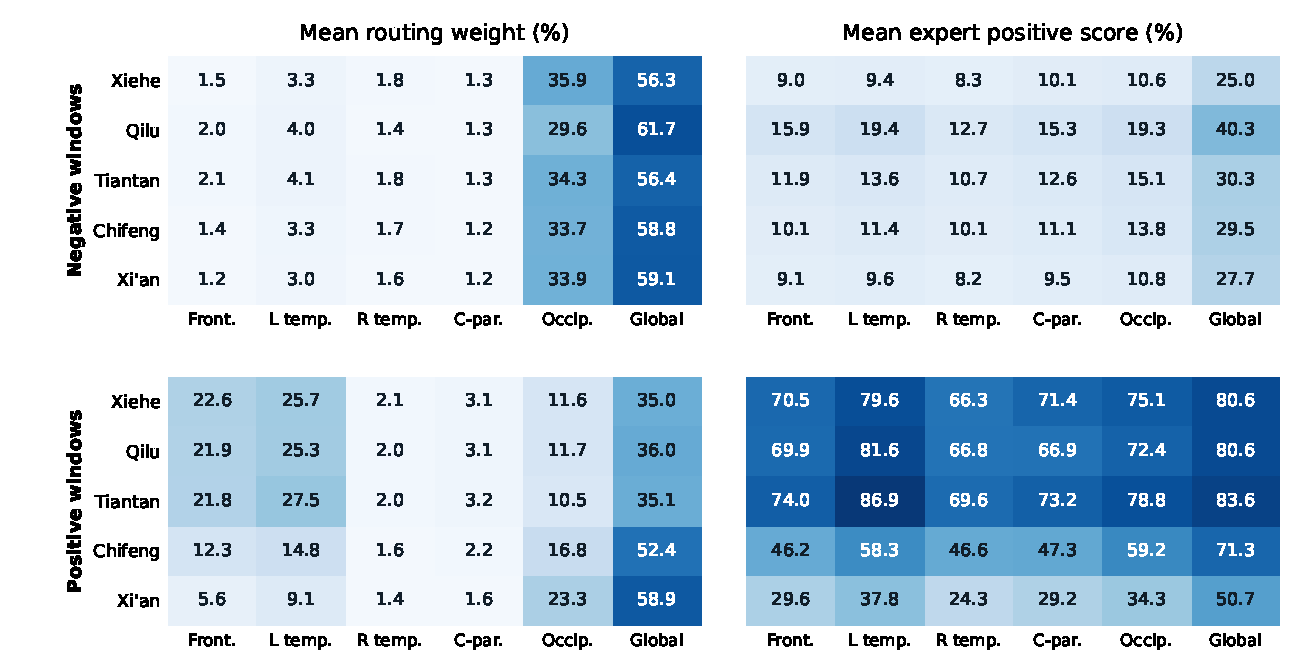
\includegraphics[width=0.94\textwidth]{figures/hospital-experts.pdf}
\caption{Activity by site and true label (\%). The left panels show routing mass, which sums to 100\% per row before rounding. The right panels show each head's positive score. Color scales are shared across label strata within each column.}\label{fig:hospital-experts}
\end{figure}

\begin{table}[ht]
\caption{Source validation activity (\%). Top share is the fraction of windows on which the expert receives the largest four-view mean routing weight.}\label{tab:expert-source}
\centering\small
\begin{tabular}{@{}lrrrrrr@{}}
\toprule & \multicolumn{2}{c}{Mean routing weight} & \multicolumn{2}{c}{Top share} & \multicolumn{2}{c}{Mean expert positive score}\\
\cmidrule(lr){2-3}\cmidrule(lr){4-5}\cmidrule(l){6-7}
Expert & Negative & Positive & Negative & Positive & Negative & Positive\\ \midrule
\inputrows tables/source_experts.tex
\bottomrule
\end{tabular}
\end{table}

On Xiehe negatives, the global and occipital experts receive 56.25\% and 35.90\% of routing mass. On positives the global share falls to 34.95\%, while left-temporal and frontal weights reach 25.68\% and 22.58\%. The right-temporal expert's own positive score rises from 8.27\% to 66.29\% despite receiving only about 2\% of the routing mass.

The global expert leads on negatives at all four external sites (56.41--61.68\%). On positives, Qilu and Tiantan assign about one quarter of the mass to the left-temporal expert. Xi'an assigns it 9.14\% and the global expert 58.93\%. The global expert's positive score on Xi'an positives averages 50.68\% versus 80.61\% on Xiehe. These shifts accompany lower Xi'an recall and do not establish which expert caused an error.

The aggregate file includes per-seed counts, routing-weight quartiles, native-view means and the mean signed weighted margin, $\frac14\sum_v\pi_{jv}(\ell_{jv,1}-\ell_{jv,0})$. Equation~\eqref{eq:full} also uses probability pooling, history and corrections. These summaries quantify core behavior; they do not identify the F1 effect of deleting an expert or localize a waveform to a brain region.
